\section{因果推断导论部分}\label{SecCausalInference}
\begin{center}
    Instructor: Wanlu Deng
\end{center}



\subsection{Neyman-Rubin Potential Outcome Framework}
    Neyman-Rubin Framework\index{Neyman-Rubin Framework} (Donald B.Rubin, 1978), also called Potential Outcome Framework\index{Potential Outcome Framework} is based on \textbf{counter-factual outcome} inference to judge causal effect. 


% \begin{point}
%     Motivation of N-R Model: Difference Between `Correlation' and `Causality'
% \end{point}
    
%         Assume we now has a set of $ \{(W_i,Y_i)\} $ where $ W_i $ happens before $ Y_i $ and $ i $ for $ i^\mathrm{th}  $ object.
    
%         \begin{itemize}[topsep=2pt,itemsep=0pt]
%             \item \textbf{Correlation} describes the relation between $ W_i $ and $ Y_i $;
%             \item while \textbf{Causality} describes the relation between $ Y_i $ and some \textbf{unseen}  $ \tilde{Y}_i $ corresponding to \textbf{What If } $ W_i $ takes another value.
%         \end{itemize}
        
%         Their difference is significant, correlation is mostly based on objective data, while causality contains a lot about how we \textbf{`imagine'} what did not happen, and compare to reality. The $ Y_i-\tilde{Y}_i $ is causal effect (Note that they both has $ _i $, acting on the same object, the different causal effect on different unit also make it not so useful to increase sample size).

\subsubsection{Description of Causal Effect and Challenge}
    Causality concerns `what would happen when \textbf{an action} is applied to \textbf{a unit}'. Here the `unit' is how causality is different from correlation.
\begin{itemize}[topsep=2pt,itemsep=0pt]
    \item A unit is the physical object at that specific time, which is similar to the event in Einstein's relativity.\footnote{Which means that one object at different time ($ (x,t) $ \& $ (x,t') $) is not the same unit (event). However if the assumption of time independency is valid, then object in different time could be the same unit (usually less resonable for human subjects).}
    \item An action is the treatment/intervention that could be \textbf{potentially} applied to the unit. 
\end{itemize}

    In this section we mainly focus on cases with binary intervention, i.e.\footnote{Habitually we denote the more `active' intervention as treatment, but in mathematical form they are symmetric.}
    \begin{align}
        \{\mathrm{treatment},\,\mathrm{control} \}=\{1,0\} 
    \end{align}

\begin{point}
    Potential Outcome
\end{point}

    With this notation, the causal effect could be expressed by the \textbf{estimand} as follows by  comparing the \textbf{potential outcomes}, here's a commonly used form:
    \begin{align}
        \tau:=Y_\mathrm{treatment} -Y_\mathrm{control} :=Y(1)-Y(0)
    \end{align}

    To estimate the causal effect (on a unit), we need to obtain both potential outcomes of $ Y(1) $ and $ Y(0) $, but in the real world we can only observe one of them, say, the patient took the medicine, and we got $ Y(1) $, while $ Y(0) $ is missing.

    Relevant Notation:


    \begin{itemize}[topsep=2pt,itemsep=0pt]
        \item \textbf{Unit}: The atomic object in causal inference. $ i=1,2,\ldots,N $
        \item \textbf{Treatment} $ W_i $: (possible) assignment.
        \begin{itemize}[topsep=2pt,itemsep=0pt]
            \item Treatment Group: Set of $ \{\mathrm{Unit}_i|W_i=1\} $;
            \item Controlled Group: Set of $ \{\mathrm{Unit}_i|W_i=0 \} $.
        \end{itemize}
        \item \textbf{Potential Outcome} (PO) $ Y_i $\index{PO (Potential Outcome)}: For each unit with action  treatment(or control), the potential outcome $ Y(W=w),\,w=0,1 $ is the `Eigen Outcome' of the model, despite of what really happens. It can be seen as what would happen when the operation had not been done.
        \item \textbf{Observed Outcome} $ Y_i^\mathrm{obs}  $: The actually happened outcome, $ Y_i^\mathrm{obs}=Y_i(W=w_\mathrm{REAL\_CASE}):=Y_i(W=w_i^\mathrm{obs} ) $.
        
        \item \textbf{Missing Outcome} $ Y_i^{\mathrm{mis} } $: The potential outcome when the $ w_i^\mathrm{mis}:= !w_i^\mathrm{obs}  $ would have been operated (it does exist but we cannot observe the `world-line' where $ w^{\mathrm{mis} }_i $ was operated, thus is unknown to us), $ Y_i^{\mathrm{mis} }=Y_i(W_i=1-w_\mathrm{REAL\_CASE}):=Y_i(W_i=w_i^{\mathrm{mis} }) $ 
        \begin{align}
            Y^\mathrm{obs} _i=Y_i(W_i^\mathrm{obs} )=&\begin{cases}
                Y_i(1)&W_i=1\\
                Y_i(0)&W_i=0
            \end{cases}\\
            Y^{\mathrm{mis} }_i=Y_i(1-W_i^\mathrm{obs} )=&\begin{cases}
                Y_i(0)&W_i=1\\
                Y_i(1)&W_i=0
            \end{cases}
        \end{align}
        or in condensed notation
        \begin{align}
            \begin{bmatrix}
                Y^\mathrm{obs}_i\\
                Y^\mathrm{mis}_i  
            \end{bmatrix} = \begin{bmatrix}
                W_i&1-W_i\\
                1-W_i&W_i
            \end{bmatrix}\begin{bmatrix}
                Y_i(1)\\ Y_i(0)
            \end{bmatrix}\Leftrightarrow\begin{bmatrix}
                Y_i(1)\\ Y_i(0)
            \end{bmatrix} = \begin{bmatrix}
                W_i&1-W_i\\
                1-W_i&W_i
            \end{bmatrix}\begin{bmatrix}
                Y^\mathrm{obs}_i\\
                Y^\mathrm{mis}_i  
            \end{bmatrix}
        \end{align}
        
        
        \item \textbf{Causal Effect}\index{Causal Effect} $ \tau_i $ (defined by difference of PO): Difference between potential outcome, $ \tau_i=Y_i(W_i=1)-Y_i(W_i=0)=Y_i(1)-Y_i(0) $
        \item \textbf{Pre-Treatment Variables / Covariates} $ X_i $\index{Pre-Treatment Variable}\index{Covariate}: Some background elements that might attribute to treatment selection/potential outcome. Anyway they may cause confusion to causal inference. For example, the gender of patients $ X_i\in\{\mathrm{female}, \mathrm{male}  \}:=\{1,0\} $.
        \item \textbf{Subgroup}: Treatment/Contorl group could be further divided in subgroup according to covariates, e.g. categorical covariates $ X_i\in\mathcal{X} $
        \begin{align}
            \{(X_i,Y_i,W_i)\}=\bigotimes_{\xi \in\mathcal{\mathcal{X}}}\{(Y_i,W_i)\}_{i:X_i=\xi }
        \end{align}
    \end{itemize}

    With the above basic notation, a dataset / sample can be expressed as
    \begin{align}
        \mathcal{D}=\{(X_i,Y_i,W_i)\}_{i=1}^N 
    \end{align}
    

\begin{point}
    Assignment Mechanism and Super Population\index{Finite Sample}\index{Super Population}
\end{point}

\begin{itemize}[topsep=2pt,itemsep=0pt]
    \item Our observation sample is a \textbf{finite sample} $\{X_i,Y_i\}_{i=1}^N $ in which $ Y_i $ is perceived fixed as potential outcome. And the above notation are studying the causal information within the finite sample. The randomness of the causal effect in the sample is the \textbf{assignment mechanism}\index{Assignment Mechanism} $ W_i\sim f_{W|X,Y} $. i.e. in finite sample, POs are fixed and actually different assignment mechanisms give randomized data (in a finite sample). So if we can control the assignment mechanism $ W|Y,X $, which is the case for randomized experiment, then the assignment mechanism can help estimate the missing values.   
    Some widely used mechanism includes Completely Randomized Experiment, Stratified Randomized Experiment, Pairwise Randomized Experiment, etc. Proper assignment can help avoid the influence of covariants (recall Simpson's Paradox).
    \item Before that, the finite sample of $ \{X_i,Y_i\}_{i=1}^N $ is drawn from a \textbf{super population} with some distribution.
\end{itemize}

    To summarize, The whole model has 2 stages of randomness: sampling from super population, and assign treatment to the finite sample.
\begin{align}
    \text{Super Population}\xrightarrow[\text{sample }N]{f_{X}, f_{Y|X}}\text{Finite Sample }\{X,Y\}\xrightarrow[\text{assignment}]{f_{W|X,Y}}\text{Observation }\mathcal{D}=\{X,Y,W\}
\end{align}


\subsubsection{Assumptions}

The null model is complicated, say, there could be multiple PO levels / interference between assignments / complex assignment mechanism, etc. There are some basic assumptions to help simplified the model.

\textbf{Note}: In actual usage of causal model, the assumptions should be checked.  

\begin{itemize}[topsep=2pt,itemsep=0pt]
    \item \textbf{SUTVA}:\index{SUTVA (Stable Unit Treatment Value Assumption)} To solve the problem of omitted treatment (e.g. $ Y_i\in\{Y_i(0),Y_i(1),Y_i(2)\} $), and the intervention between units (e.g. $ Y_i(W_{j=1:N}) $) to simplify the model, we usually put the assumption of SUTVA, which has two components:
    \begin{itemize}[topsep=2pt,itemsep=0pt]
        \item No Interference
        \begin{align}
            Y_i(W_{j=1:N})=Y_i(W_i) 
        \end{align}
        \item No Hidden Variation of Treatment:
        \begin{align}
            Y_i(W_{j=1:N})=Y_i(W_i)\in\{Y_i(1),Y_i(0)\},\quad W_i\in \{1,0\}:=\mathbb{T}_i=\mathbb{T}
        \end{align}
    \end{itemize}
    \item \textbf{Regular Assignment Mechanisms (RAM)} \index{RAM (Regular Assignment Mechanisms)}
    \begin{itemize}[topsep=2pt,itemsep=0pt]   
        \item \textbf{Individualistic Assignment}: Assignment probability of each unit does \textbf{not} depends on the covariants and PO of other units:
        \begin{align}
            \mathbb{P}(W_i=w_i|X,Y(1),Y(0))=&\mathbb{P}\left( W_i=w_i|X_i,Y_i(1),Y_i(0) \right) \\
            =&\mathbb{P}(W_i|X_i,Y_i(1),Y_i(0))^{w_i}(1-\mathbb{P}(W|X_i,Y_i(1),Y_i(0)))^{1-w_i},\,\forall i=1,2,\ldots,N
        \end{align}

        Sometimes for simplification, denoted as
        \begin{align}
            \mathbb{P}_i(W=1|X,Y(1),Y(0)):=q(X,Y(1),Y(0)) 
        \end{align}        
        % Under individualistic assignment assumption, propensity score is simplified:
        % \begin{align}
        %      e(x)=\dfrac{1}{N(x)}\sum_{i:X_i=x}P(W=1|X,Y(1),Y(0))=\dfrac{1}{N(x)}\sum_{i:X_i=x}P(W=1|X_i,Y_i(1),Y_i(0))
        % \end{align}
        
        \item \textbf{Probabilistic Assignment}: Probility for both $ W_i=1 $ and $ W_i=0 $ are non-zero (to ensure a reasonable causal model)
        \begin{align}
            0<\mathbb{P}(W|X,Y(1)Y(0))<1,\,\forall X,Y(1),Y(0) 
        \end{align}
        
        \item \textbf{Unconfounded Assignment}: Assignment mechanism is independent of PO
        \begin{align}
            \mathbb{P}(W|X,Y(1),Y(0))=\mathbb{P}(W|X)
        \end{align}

        when $ q(X,Y) $ mentioned above does \textit{not} involve $ Y $, i.e. with unconfoundedness, it is denoted as \textit{propensity score}\index{Propensity Score}.
        \begin{align*}
            q(X,Y) := e(X),\quad \text{case } W\independent Y\big| X
        \end{align*}

        Note: Unconfoundedness is \textit{not} testable (always invloves the missing value $ Y^\mathrm{mis}  $). We can only pre-design it (randomized experiment) or make it an appropriate assumption (RAM).
    \end{itemize}
\end{itemize}


    
\begin{point}
    With all the above assumptions, assignment mechanism can be simplified in the following form:
\end{point}

\begin{align}
    \text{Assignment Mechanism:}\,&\mathbb{P}(W|X,Y(1),Y(0))=\dfrac{1}{Z}\prod_{i=1}^N e(X_i)^{W_i}(1-e(X_i))^{1-W_i}\\
\end{align}

% \subsubsection{Causal Effect Measurement}


% \begin{itemize}[topsep=2pt,itemsep=0pt]
%     \item \textbf{ACE}: Average Causal Effect (ACE) of the whole population:\footnote{Some uses the name Average Treatment Effect (ATE), the following parts are similar for ACT}
%     \begin{align}
%         \mathrm{ATE}=E(Y(1)-Y(0))  
%     \end{align}

%     Estimand:
%     \begin{align}
%         \hat{\mathrm{ATE} }=\dfrac{1}{N}\sum_{i=1}^N(Y_i(1)-Y_i(0)) 
%     \end{align}

%     \item \textbf{ATT}/\textbf{ATC}: Average Treatment Effect of Treated/Controlled Group (ATT/ATC):
%     \begin{align}
%         \mathrm{ATT}=E(Y(1)|w=1)-E(Y(0)|w=1)  \qquad \mathrm{ATC}=E(Y(1)|w=0)-E(Y(0)|w=0) 
%     \end{align}

%     Estimand:
%     \begin{align}
%         \hat{\mathrm{ATT} }=\dfrac{1}{N_t}\sum_{i:w_i=1}(Y_i(1)-Y_i(0))\qquad \hat{\mathrm{ATC} }=\dfrac{1}{N_c}\sum_{i:w_i=0}(Y_i(1)-Y_i(0)) 
%     \end{align}
    
    
%     \item \textbf{CATE}: Conditional Average Treatment Effect (CATE): `Conditional' for `given covariant $ X $'
%     \begin{align}
%         \mathrm{CATE}_x=E(Y(1)|X=x)-E(Y(0)|X=x)
%     \end{align}
%     Estimand: (Denote \# $ X_i=x $ as $ N(x) $)
%     \begin{align}
%         \hat{\mathrm{CATE} }=\dfrac{1}{N(x)}\sum_{i:X_i=x}(Y_i(1)-Y_i(0)) 
%     \end{align}
    
    
%     % \item \textbf{ITE}: Individual Treatment Effect:
%     % \begin{align}
%     %     \mathrm{ITE}_i=Y_i(W=1)-Y_i(W=0)  
%     % \end{align}
% \end{itemize}

%     Where in Estimands, we only know one of $ Y_i(1)/Y_i(0) $ as $ Y^\mathrm{obs}  $, the $ Y^{\mathrm{mis} } $ needs to be \textbf{predicted} (or at least we need to know about the property).

    


    \begin{point}
        Data Example
    \end{point}
    
        \begin{table}[H]
            \centering
            \renewcommand\arraystretch{1}
            \caption{Illustration of Causal Data}
            \begin{tabular}{cccccc}
                \hline
                \hline
                &\multicolumn{2}{c}{Potential Outcomes}&Assignment&Observation&Causal Estimand\\
                \cline{2-3}
                Unit $ i $&$ Y_i(1) $&$ Y_i(0) $&$ W_i $&$ Y^\mathrm{obs}_i  $&$ Y_i(1)-Y_i(0) $\\
                \hline
                \# 1&$ \color{brown}Y_1(1) $&$ \color{gray}Y_1(0) $&$ W_1={\color{brown}1} $&$ Y^\mathrm{obs}_1=\color{brown}Y_1(1)  $&$ {\color{brown}Y_1(1)}-{\color{gray}Y_1(0)} $\\
                \# 2&$ \color{gray}Y_2(1) $&$ \color{brown}Y_2(0) $&$ W_2={\color{brown}0} $&$ Y^\mathrm{obs}_2=\color{brown}Y_2(0)  $&$ {\color{gray}Y_2(1)}-{\color{brown}Y_2(0)} $\\
                \# 3&$ \color{gray}Y_3(1) $&$ \color{brown}Y_3(0) $&$ W_3={\color{brown}0} $&$ Y^\mathrm{obs}_3=\color{brown}Y_3(0)  $&$ {\color{gray}Y_3(1)}-{\color{brown}Y_3(0)} $\\
                \# 4&$ \color{brown}Y_4(1) $&$ \color{gray}Y_4(0) $&$ W_4={\color{brown}1} $&$ Y^\mathrm{obs}_4=\color{brown}Y_4(1)  $&$ {\color{brown}Y_4(1)}-{\color{gray}Y_4(0)} $\\
                $ \vdots $&$ \vdots $&$ \vdots $&$ \vdots $&$ \vdots $&$ \vdots $\\
                \hline
                \hline
            \end{tabular}
            \label{}
        \end{table}
    

    


\subsection{Inference to Causal Effect in Completely Randomized Experiment}

First we focus on the randomness in finite sample, i.e. randomness of assignment mechanism. Specifically we usually consider the case of Completely Randomized Experiment (CRE)\index{CRE (Completely Randomized Experiment)}: $ N_t $ in $ N $ items are given treatment and $ N_c=N-N_t $ in $ N $ are given control, and the assignment is given \textbf{randomly}. 
\begin{align}
    \mathbb{P}\left( W|X,Y \right)=1\bigg/\binom{N}{N_\mathrm{t} },\quad W\in\mathbb{W}^\mathrm{CRE}:=\left\{W:\,\sum_{i=1}^NW_i=N_\mathrm{t}\right\}
\end{align}

The assumption of CRP is important in causal inference because it fixes the gap between $ Y^\mathrm{obs}  $ and $ Y^\mathrm{mis} $ by randomly assign treatment/control.


\subsubsection{Fisher's Exact $ p $-value}

Test of Fisher's Sharp Null Hypothesis\index{Fisher's Sharp Null Hypothesis}:
\begin{align}
    H_0:\tau_i=0,\,\forall i=1,2,\ldots,N  \leftrightsquigarrow H_a:\,\exists j\,s.t. \tau_j\neq 0
\end{align}

With the hypothesis, we could fill in all the $ Y^\mathrm{mis}  $ by $ Y^\mathrm{mis}_i=Y^\mathrm{obs}_i   \,\forall i$. And by traversing all possible $ \tilde{W} $ assignments and calculate corresponding $ \tau_{\tilde{W}} $, we could calculate the Fisher's exact $ p $-value
\begin{align}
     \hat{p}={\#(|\tau_{\tilde{W}}|\geq |\tau_{W}|)}\bigg/\binom{N}{N_t}
\end{align}

Comments:
\begin{itemize}[topsep=2pt,itemsep=0pt]
    \item Since the basic idea is traversing all $ W $, so it could be applied to differenet deigns of $ \tau $, say 
    \begin{align}\label{EqaFEPStatistics}
        \hat{\tau}^\mathrm{diff}=&|\bar{Y}_\mathrm{t}^\mathrm{obs}-\bar{Y}_\mathrm{c}^\mathrm{obs}|\\
        \hat{\tau}^\mathrm{median}=&|\mathrm{med}_\mathrm{t}(Y^\mathrm{obs} )-\mathrm{med}_\mathrm{c}(Y^\mathrm{obs} )    |  \\
        \hat{\tau}^{t\text{-}\mathrm{stat} }=&\left| \dfrac{\bar{Y}_\mathrm{t}^\mathrm{obs}-\bar{Y}_\mathrm{c}^\mathrm{obs}}{\sqrt{ s_\mathrm{t}^2/N_t+s_\mathrm{c}^2/N_c   }} \right| \\
        \hat{\tau}^\mathrm{rank}=&|\bar{R}_\mathrm{t}-\bar{R}_\mathrm{c}|,\quad R_i=\sum_{j=1}^N\left(\mathbb{I}_{Y_j<Y_i}+\dfrac{1}{2}\mathbb{I}_{Y_j=Y_i}\right)-\dfrac{N}{2}\\
        \hat{\tau}^\mathrm{reg}=&\mathop{\arg\min}\limits_{\tau:(\beta _0,\beta _X,\tau)}\sum_{i=1}^N\left(Y_i^{\mathrm{obs}}-\beta _0-\tau W_i-X_i'\beta _X\right)^2  
    \end{align}
    Or even some other specially designed statistics on e.g. difference in variance
    \begin{align}
        \hat{\tau}^{var}=&\hat{var}^\mathrm{obs}_\mathrm{t} \big/\hat{var}^\mathrm{obs}_\mathrm{c}     
    \end{align}
    \item High computation complexity for large $ N $. e.g. for $ N_t\approx \dfrac{N}{2} $
    \begin{align}
        \mathrm{flops}\sim \binom{N}{N_t}\sim 2^N 
    \end{align}
    \item Random simulation for large $ N $: the $ p $-value is actually
    \begin{align}
        \hat{\mathbb{P}}\left( \text{more extreme }\hat{\tau} \right)=\hat{\mathbb{E}}\left[\mathbf{1}(\text{more extreme }\hat{\tau})\right] 
    \end{align}
    which can be approached by random sampling
    \begin{align}
        \hat{p}={\#(|\tau_{\tilde{W}}|\geq |\tau_{W}|)}\Big/{\#(\text{sample})}
   \end{align}
    \item A fiducial interval can be constructed. But generally speaking the hypothesis testing just help reject the sharp hypothesis, but cannot help determine the casual effect strength.
\end{itemize}

    
\subsubsection{Neyman's Repeated Sampling Approach}

Neyman's method uses the distribution of $ W $ for completely randomized experiment to obtain the property of the finite sample estimator
\begin{align}
    \hat{\tau}_\mathrm{fs}=\bar{Y}_\mathrm{t}^\mathrm{obs}-\bar{Y}_\mathrm{c}^\mathrm{obs}= \dfrac{1}{N_\mathrm{t} }\sum_{i=1}^N W_iY_i(1)-\dfrac{1}{N_\mathrm{c} } \sum_{i=1}^N(1-W_i)Y_i(0)   
\end{align}

\begin{itemize}[topsep=2pt,itemsep=0pt]
    \item Property
    \begin{align}
        \mathbb{E}_W\left[ \hat{\tau}_\mathrm{fs}  \right] = & \tau_\mathrm{fs}=\dfrac{1}{N}\sum_{i=1}^NY_(1)-Y_i(0) \\
        var_W(\hat{\tau}_\mathrm{fs} )=&\dfrac{S_\mathrm{t} ^2}{N_\mathrm{t} }+\dfrac{S_\mathrm{c} ^2}{N_\mathrm{c} }-\dfrac{S^2_{\mathrm{tc} }}{N}\\
        =&\dfrac{N_\mathrm{c} }{NN_\mathrm{t} }S_\mathrm{t} ^2+\dfrac{N_\mathrm{t} }{NN_\mathrm{c} }S_\mathrm{c}^2+\dfrac{2}{N}\rho _{\mathrm{tc} }S_\mathrm{t}S_\mathrm{c}    \\
        &\begin{cases}
            S_\mathrm{t}^2=\dfrac{1}{N-1}\sum_{i=1}^N(Y_i(1)-\bar{Y}(1))^2\\
            S_\mathrm{c}^2=\dfrac{1}{N-1}\sum_{i=1}^N(Y_i(0)-\bar{Y}(0))^2\\
            S_\mathrm{tc}^2=\dfrac{1}{N-1}\sum_{i=1}^N\left([Y_i(1)-Y_i(0)]-[\bar{Y}(1)-\bar{Y}(0)]\right)^2=S_\mathrm{t}^2+S_\mathrm{c}^2-2\rho _\mathrm{tc}S_\mathrm{t}S_{\mathrm{c} }    \\
            \rho _\mathrm{tc}=\dfrac{1}{(N-1)S_\mathrm{t}S_{\mathrm{c} } }\sum_{i=1}^N\left(Y_i(1)-\bar{Y}(1)\right)\left(Y_i(0)-\bar{Y}(0)\right) 
        \end{cases}
    \end{align}
    \item Estimator
    \begin{align}
        \hat{\tau}_\mathrm{fs}= & \bar{Y}_\mathrm{t}^\mathrm{obs}-\bar{Y}_\mathrm{c}^\mathrm{obs}\\
        \hat{var}(\hat{\tau}_\mathrm{fs} )=&\dfrac{s^2_\mathrm{t} }{N_t}+\dfrac{s^2_\mathrm{c} }{N_c}\\
        \hat{var}_\rho (\hat{\tau}_\mathrm{fs} )=&\dfrac{N_\mathrm{c} }{NN_\mathrm{t} }s_\mathrm{t} ^2+\dfrac{N_\mathrm{t} }{NN_\mathrm{c} }s_\mathrm{c}^2+\dfrac{2}{N}\rho s_\mathrm{t}s_\mathrm{c},\,\, -1\leq \rho \leq 1 \\
        \mathrm{e.g.}\hat{var}_{\rho =1}(\hat{\tau}_\mathrm{fs} )=& \dfrac{s^2_\mathrm{t} }{N_t}+\dfrac{s^2_\mathrm{c} }{N_c}-\dfrac{(s_\mathrm{t}-s_\mathrm{c}  )^2}{N}\leq \hat{var}(\hat{\tau}_\mathrm{fs} )\\ 
        &\begin{cases}
            s^2_\mathrm{t}=\dfrac{1}{N_t-1}\sum_{i:W_i=1}\left(Y_i^\mathrm{obs} -\bar{Y}^\mathrm{obs}_\mathrm{t}  \right)^2 \\
            s^2_\mathrm{c}=\dfrac{1}{N_c-1}\sum_{i:W_i=0}\left(Y_i^\mathrm{obs} -\bar{Y}^\mathrm{obs}_\mathrm{c}  \right)^2
        \end{cases}
    \end{align}

    i.e. $ \hat{var}(\hat{\tau}_\mathrm{fs} ) $ provides an upper bound of $ \hat{var}_\rho (\hat{\tau}_\mathrm{fs} ) $ (equal when $ \rho =1 $). And $  \hat{var}(\hat{\tau}_\mathrm{fs} )  $ also acts as the estimator at $ \tau_i=\mathrm{const},\,\forall i $.\footnote{Actually in this case we should have $ s_\mathrm{t}=s_\mathrm{c}:=s    $ and the estimator reduces to $ \hat{var}(\hat{\tau}_\mathrm{fs} )=s^2(1/N_\mathrm{t}+1/N_\mathrm{c}  ) $}

    
    
    \item Confidence Interval
    
    \begin{align}
        \mathrm{CI}=&  \hat{\tau}_\mathrm{fs}\pm N_{\alpha /2}\sqrt{\hat{var}(\hat{\tau}_\mathrm{fs} )}  \\
        \mathrm{CI}_\rho =&  \hat{\tau}_\mathrm{fs}\pm N_{\alpha /2}\sqrt{\hat{var}_\rho (\hat{\tau}_\mathrm{fs} )}  
    \end{align}
    
    where the version with pre-specified $ \rho  $ is applied to improve accuracy, if we have prior knowledge about $ \rho_\mathrm{tc}   $. 
    
    \item Hypothesis Testing
    \begin{align}
        H_0:\bar{Y}(1)-\bar{Y}(0)=0\leftrightsquigarrow H_a: \bar{Y}(1)-\bar{Y}(0)\neq 0
    \end{align}

    and $ t $-test
    \begin{align}
        T=\dfrac{\hat{\tau}_\mathrm{fs}    }{\sqrt{\hat{var}(\hat{\tau}_\mathrm{fs} )}} \sim t_1
    \end{align}
    \item Comment on three components $ S^2_\mathrm{t}$ / $S^2_{\mathrm{c} }$ / $S^2_{\mathrm{tc} }  $: they each corresponds to the natural distribution of treatment / natrual distribution of control / variation arises from assigning on finite sample.
    
    So when dealing with the estimator under distribution of super population, in which we need to add the randomness of $ f_{X,Y} $ back, the $ S^2_\mathrm{tc}  $ term eliminates (which can be proven).
    \begin{align}
        \mathbb{E}_\mathrm{sp} \left[ \hat{\tau}_\mathrm{fs}  \right] = & \mathbb{E}_\mathrm{sp} \left[ \mathbb{E}_W \left[ \hat{\tau}_\mathrm{fs}  \right] \right] = \tau_\mathrm{sp}  \\
        var_\mathrm{sp} (\hat{\tau}_\mathrm{fs} )=&\mathbb{E}_\mathrm{sp} \left[( \bar{Y}_\mathrm{t} ^\mathrm{obs}-\bar{Y}_\mathrm{c}^\mathrm{obs}-\mathbb{E}_\mathrm{sp} \left[ \bar{Y}(1)-\bar{Y}(0) \right]    )^2 \right] = \dfrac{\sigma _\mathrm{t}^2 }{N_t}+\dfrac{\sigma _\mathrm{c}^2 }{N_c}\\
        \hat{var}_\mathrm{sp}(\hat{\tau}_\mathrm{fs} )=&\dfrac{s_\mathrm{t}^2 }{N_t}+\dfrac{s_\mathrm{c}^2 }{N_c} 
    \end{align}

    where $ \sigma ^2_\cdot $ is the variance under the distribution of super population $ Y|X $, $ X $.
    \begin{align}
         \sigma _\mathrm{t}^2(x)=&var_{\mathrm{sp}:\,Y|X}\left(Y(1)|X=x\right) ,& \sigma _\mathrm{t}^2=&var_\mathrm{sp}\left(Y(1)\right)\\
         \sigma _\mathrm{c}^2(x)=&var_{\mathrm{sp}:\,Y|X}\left(Y(0)|X=x\right) ,& \sigma _\mathrm{c}^2=&var_\mathrm{sp}\left(Y(0)\right)\\
         \sigma _\mathrm{ct}^2(x)=&var_{\mathrm{sp}:\,Y|X}\left(Y(1)-Y(0)|X=x\right) ,& \sigma _\mathrm{ct}^2=&var_\mathrm{sp}\left(Y(1)-Y(0)\right)
    \end{align}
    
    

    
\end{itemize}


\subsubsection{Regression Methods}

Regression methods in Potential Outcome Framework is used to introduce covariates and lower the variance estimation, the idea is similar to variance decomposition in ANOVA.

\begin{point}
    Requisite Knowledge: M-Estimator\index{M-Estimator (Maximization Estimator)}
\end{point}

With data $ \mathcal{D}_n $ given, parameter estimation problem can usually be expressed in a \textbf{M}aximization problem with linear combination target function $ Q_n(\theta ;\mathcal{D}_n) $ 
\begin{align}
    \hat{\theta }_n=\mathop{\arg\max}\limits_{\theta } Q_n(\theta;\mathcal{D}_n )
\end{align}
e.g. for regression estimation $ Y=X\beta + \varepsilon  $, $ \mathcal{D}_n=\{x_i,y_i\}_{i=1}^n=(X,Y) $
\begin{itemize}[topsep=2pt,itemsep=0pt]
    \item OLS quadratic form $ \theta = \beta $ 
    \begin{align}
        Q_n(\theta ) := -\dfrac{1}{n}\sum_{i=1}^n\left(y_i-x_i'\beta \right)^2=-\dfrac{1}{n}(Y-X\beta )'(Y-X\beta )
    \end{align}
    \item MLE form with $ \varepsilon \sim f(\varepsilon ; \phi ) $, and $ \theta =(\beta ,\phi ) $
    \begin{align}
        Q_n(\theta ) :=\dfrac{1}{n} \sum_{i=1}^nf\left(y_i-x_i'\beta ; \phi  \right)
    \end{align} 
\end{itemize}

    Denote the ground truth $ \theta ^* $, and the M-Estimator $ \hat{\theta }_n $ that maximizes $ Q_n $. Then
    \begin{align}
        \theta ^* =& \mathop{\arg\max}\limits_{\theta } \mathbb{E}_{\mathcal{D}}\left[ Q(\theta ; \mathcal{D}) \right]\\
        \hat{\theta }_n=&\mathop{\arg\max}\limits_{\theta } Q_n\\
        \text{with }&Q_n\to \mathbb{E}\left[ Q \right] \Rightarrow \hat{\theta }_n\to \theta ^*
    \end{align}

    The solution $ \hat{\theta }_n $ is obtained at $ \dfrac{\partial^{} Q_n(\theta )}{\partial \theta ^{}} =0$, so we first focus on first order derivative
    \begin{align}
        \psi_n(\theta;\mathcal{D}_n ) := \dfrac{\partial^{} Q_n(\theta;\mathcal{D}_n )}{\partial \theta ^{}},\quad \hat{\theta }_n=\mathop{\arg}\limits_{\theta }(\psi_n(\theta ;\mathcal{D}_n)=0 )
    \end{align}

    Note: a more important reason we study the property of $ \psi_n(\theta ;\mathcal{D}_n) $ is that: we do \textbf{not} have an explicit expression of $ \hat{\theta }_n$ because it's just a maximizer. $ \psi_n(\theta ;\mathcal{D}_n) $ together with taylor expansion provide us with an approach to (asymptotically) express $ \hat{\theta }_n $ explicitly.
    % $ \hat{\theta }_n $ and $ \psi(\hat{\theta }_n;\mathcal{D}) $ are both statistics. From\hyperlink{ContinuousMapping}{continuous mapping thm.} we have\footnote{Here the derivation seems not quite rigorous, but anyway I think it makes sense.}
    % \begin{align}
    %     0=\psi(\hat{\theta }_n;\mathcal{D})\xrightarrow[]{d} \psi(\theta ^*;\mathcal{D})
    % \end{align}

    with LLN, we have
    \begin{align}
        \psi_n(\theta ^*;\mathcal{D}_n)\xrightarrow[]{\mathrm{d} } \mathbb{E}\left[ \psi(\theta ^*) \right] =0  
    \end{align}

    with CLT, $ \psi_n(\theta ^*,\mathcal{D}_n) $ is a statistic asymptotically distributed normally:
    \begin{align}
        \sqrt{n}\left(\psi_n(\theta ^*;\mathcal{D}_n)-\mathbb{E}\left[ \psi(\theta ^*;\mathcal{D}) \right]\right)=\sqrt{n}\psi_n(\theta ^*;\mathcal{D}_n) \xrightarrow[]{d} N(0,\Sigma _{\psi})
    \end{align}

    Taylor series of $ \psi_n(\, \cdot \, ;\mathcal{D}_n) $ at $ \hat{\theta }_n $:
    \begin{align}
        \psi_n(\theta ^*;\mathcal{D}_n)=& 0 + \dfrac{\partial^{} \psi_n(\theta =\hat{\theta}_n;\mathcal{D}_n)}{\partial \theta ^{}}\left(\theta ^*-\hat{\theta }_n\right)+O((\theta ^*-\hat{\theta }_n)^2)\\
        \Rightarrow \left(\hat{\theta }_n-\theta ^*\right)\approx & \left( \dfrac{\partial^{} \psi_n(\theta =\hat{\theta}_n;\mathcal{D}_n)}{\partial \theta ^{}}\right)^{-1}\psi_n(\theta ^*;\mathcal{D}_n)\\
        \Rightarrow \hat{\theta }_n\xrightarrow[]{d} &N(\theta ^*,\Gamma ^{-1}\Sigma _{\psi}\Gamma ^{-1}\big/n ),\qquad \Gamma :=\dfrac{\partial^{} \psi_n(\theta =\hat{\theta}_n;\mathcal{D}_n)}{\partial \theta ^{}}
    \end{align}

    and specifically if $ Q_n(\theta ;\mathcal{D}) $ is a log-likelihood, then $ \psi(\theta ;\mathcal{D}) $ here is Score function in \autoref{EqaScoreFunctionForMLE}. And $ \Sigma _\psi=I(\theta )  $ is Fisher Information in \autoref{EqaFisherInformation}. With the nice property of Fisher Information $ I(\theta )=\Sigma _{\psi}=-\mathbb{E}\left[ \Gamma  \right]  $, M-Estimator reduces to the asymptotic distribution of MLE in \autoref{EqaAsymptoticDistributionMLE}
    \begin{align}
         \hat{\theta }_n\xrightarrow[]{d} (\theta ^*,\dfrac{ I(\theta )^{-1}}{n})
    \end{align}
    
\begin{point}
    Regression Model on Super Population
\end{point}

Motivation: regression model
\begin{align}
    Y_i^\mathrm{obs}=\alpha +\tau\cdot W_i + f(X_i;\beta )+\varepsilon _i  
\end{align}
concerns a quadratic loss function of the following form:
\begin{align}
    (\hat{\alpha },\hat{\tau},\hat{\beta })_{\mathrm{ols},X}=\mathop{\arg\min}\limits_{(\alpha ,\tau,\beta )} \dfrac{1}{N}\sum_{i=1}^N\left( Y^\mathrm{obs}_i-\alpha-\tau\cdot W_i - f(X_i;\beta )\right)^2 := \mathop{\arg\min}\limits_{(\alpha ,\tau,\beta )}Q_N\left((\alpha ,\tau,\beta );\{X_i,Y_i,W_i\}_{i=1}^N\right)
\end{align}

\textbf{Note} :
\begin{itemize}[topsep=2pt,itemsep=0pt]
    \item Covariate dependency function $ f(\, \cdot \, ;\beta ) $ is a properly selected prior, e.g. linear regression $ X'\beta  $
    \item In functional form it's the same as regression (reflects correlation), the causality comes from CRE of $ W_i $.
\end{itemize}

\textbf{Solution}:
\begin{itemize}[topsep=2pt,itemsep=0pt]
    \item Model without covariates
    \begin{align}
        Y_i^\mathrm{obs} = \alpha +\tau\cdot W_i+\varepsilon _i  
    \end{align}

    OLS solution:
    \begin{align}
        \hat{\tau}_\mathrm{ols} =&\dfrac{\sum_{i=1}^N(W_i-\bar{W})(Y_i^\mathrm{obs}-bar{Y}^\mathrm{obs}  )}{\sum_{i=1}^N(W_i-\bar{W})^2}=\bar{Y}^\mathrm{obs}_\mathrm{t}-\bar{Y}^\mathrm{obs}_\mathrm{c}   \\
        \hat{\alpha }_\mathrm{ols} =&\bar{Y}^\mathrm{obs}-\hat{\tau}_\mathrm{ols} \cdot\bar{W}  \\
        var(\hat{\tau})=&\dfrac{\sigma _\mathrm{t}^2 }{N_\mathrm{t} }+\dfrac{\sigma _\mathrm{c}^2 }{N_\mathrm{c} }\\
        s^2_\mathrm{t}= \hat{\sigma }_\mathrm{t}^2=&\dfrac{1}{N-1}\sum_{i=1}^NW_i\left(Y_i^\mathrm{obs}-\hat{Y}_i^\mathrm{obs}  \right)^2=\dfrac{1}{N-1}\sum_{i=1}^NW_i\left(Y_i^\mathrm{obs}-\hat{\tau}-\hat{\alpha } \right)^2\\
        s_\mathrm{c}^2= \hat{\sigma }_\mathrm{c}^2=&\dfrac{1}{N-1}\sum_{i=1}^N(1-W_i)\left(Y_i^\mathrm{obs}-\hat{Y}_i^\mathrm{obs}  \right)^2=\dfrac{1}{N-1}\sum_{i=1}^N(1-W_i)\left(Y_i^\mathrm{obs}-\hat{\alpha } \right)^2\\
        \hat{var}(\hat{\tau}_\mathrm{ols} )=&\dfrac{s_\mathrm{t}^2 }{N_t}+\dfrac{s_\mathrm{c}^2 }{N_c}=\hat{var}(\hat{\tau}_\mathrm{fs} )
    \end{align}
    
    % Correspondance to \hyperlink{GaussMarkovAssumption}{Gauss Markov Assumption} in \autoref{SecLinearRegressionAnalysis}:
    % \begin{align}
    %     \begin{cases}
    %         \mathbb{E}\left[ \varepsilon _i|X_i,W_i \right] =0\\
    %         var(\varepsilon _i)=\sigma ^2\\
    %         \varepsilon _i \independent \varepsilon _j
    %     \end{cases}
    % \end{align}
    \item Model with Covariates and Asymptotic Property:
    \begin{align}
        Y_i^\mathrm{obs} = \alpha +\tau\cdot W_i +f(X_i;\beta)  +\varepsilon _i 
    \end{align}

    The quadratic loss $ Q_N(\, \cdot \, ) $ regression model gives a M-Estimator with ground truth as the parameters in super population
    \begin{align}
        (\alpha ,\tau,\beta )^*=\mathbb{E}_\mathrm{sp} \left[ (\alpha ,\tau,\beta ) \right]  := (\alpha_\mathrm{sp}  ,\tau_\mathrm{sp},\beta_\mathrm{sp} )
    \end{align}

    OLS with covariates gives the same optimization solution to $ \tau $ as OLS without covariate: $ \hat{\tau}_{\mathrm{ols},X }=\hat{\tau}_\mathrm{ols}\to \tau^*=\tau_\mathrm{sp}  $. And appending covariate dependency term can help \textbf{improve variance estimation} , with unbiasness property kept. 

    e.g. for linear dependency $ f(X;\beta )=X'\beta  $
    \begin{align}
        \hat{\tau}_{\mathrm{ols},X }=\hat{\tau}_{\mathrm{ols} }\to&\tau_\mathrm{sp}\\
        \sqrt{N}(\hat{\tau}_{\mathrm{ols},X }-\tau_\mathrm{sp} )  \xrightarrow[]{d} & N\left(0,(\Gamma ^{-1}\Sigma _{\psi}\Gamma ^{-1})_{22}\right)=N\left(0,\dfrac{\Sigma _{\psi,22}}{p^2(1-p)^2}\right)\\
        &\begin{cases}
            \Sigma _{\psi,22}=\mathbb{E}_\mathrm{sp} \left[\dfrac{\partial^{} Q_N(\alpha ,\tau,\beta )}{\partial (\alpha ,\tau,\beta )^{}}
            \dfrac{\partial^{} Q_N(\alpha ,\tau,\beta )}{\partial (\alpha ,\tau,\beta )'}\right]_{22}\\
            \qquad =\mathbb{E}\left[ (W_i-p)^2\left(Y^\mathrm{obs}-\alpha ^*-\tau^*W_i-X'\beta ^* \right)^2 \right] \\
            p=\bar{W}_{N\to\infty }
        \end{cases}
    \end{align}

    using the asymptotic normality, we can construct variance estimation $ \hat{var}_\mathrm{hetero} (\hat{\tau}_{\mathrm{ols} ,X})=\hat{\Sigma }_{\psi,22}\big/ \hat{p}^2(1-\hat{p})^2 $ to $ \hat{\tau}_{\mathrm{ols} ,X} $ (with heteroskedasticity)
    \begin{align}
        \hat{var}_\mathrm{hetero} (\hat{\tau}_{\mathrm{ols} ,X}) = & \dfrac{1}{N(N-\dim(X_i)-1)}\cdot\dfrac{\sum_{i=1}^N(W_i-\bar{W})^2\left(Y_i^\mathrm{obs}-\hat{\alpha}_{\mathrm{ols} ,X}-\hat{\tau}_{\mathrm{ols} ,X}W_i-X_i'\hat{\beta }_{\mathrm{ols} ,X} \right)^2}{\bar{W}^2\left(1-\bar{W}\right)^2}
    \end{align}
    
    % \item Model with Interaction Covariate
\end{itemize}

\subsubsection{Model Based Inference using Bayesian Statistics}
Motivation: how to use prior information about distribution? Basically with $ \mathbb{P}\left( W|Y,\theta  \right)  $, $ f(Y|\theta ) $, $ \pi(\theta ) $ we can construct any posterior distribution from 
\begin{align}
    f(W,Y,X)= \mathbb{P}\left( W|Y,\theta  \right)f(Y|\theta )pi(\theta )
\end{align}


\begin{point}
    Bayesian Statistics Precap
\end{point}

Estimation target: $ f(Y^\mathrm{mis}|Y^\mathrm{obs},W ) $, with assumptions
\begin{align}
    \text{CRE: }\mathbb{P}\left( W|Y,\theta  \right)=&\binom{N}{N_t} ^{-1}\\
    \text{Distribution: }\begin{pmatrix}
        Y(1)\\
        Y(0)
    \end{pmatrix}\Big|\,\theta \sim & f(Y|\theta ),\text{ say } N\left(\begin{pmatrix}
        \mu _\mathrm{t}\\
        \mu _\mathrm{c}      
    \end{pmatrix},\begin{pmatrix}
        \sigma _\mathrm{t}^2& \rho \sigma_\mathrm{t}\sigma _\mathrm{c}\\
        \rho \sigma _\mathrm{t}  \sigma _\mathrm{c}&\sigma _\mathrm{c}^2     
    \end{pmatrix}\right),\quad \theta =[\mu _\mathrm{t},\mu _\mathrm{c} ,\sigma^2_\mathrm{t},\sigma ^2_\mathrm{c} ,\rho ]\\
    \text{Prior: }\theta \sim & \pi (\theta  )\\
    \text{Transformation: }(Y^\mathrm{obs},Y^\mathrm{mis}  )=&g\left(Y(1),Y(0),W\right)
\end{align}

\begin{itemize}[topsep=2pt,itemsep=0pt]
    \item Transformation between $ Y=[Y(1),Y(0)]\mapsto [Y^\mathrm{obs},Y^\mathrm{mis}  ] $:
    \begin{align}
        {\color{brown}f\left(Y^\mathrm{obs},Y^\mathrm{mis}|W,\theta  \right)}=&f\left(Y|W,\theta \right) \left|\dfrac{\partial^{}Y(1),Y(0) }{\partial g\left(Y(1),Y(0),W\right)}\right|= \dfrac{f\left(Y,W|\theta \right)}{\int _y f\left(Y,W|\theta \right) \,\mathrm{d}y}  \left|\dfrac{\partial^{} Y(1),Y(0) }{\partial g\left(Y(1),Y(0),W\right)}\right|\\
        =& \dfrac{f\left(W|Y,\theta \right)f\left(Y|\theta \right)}{\int _y f\left(W|Y,\theta \right) f\left(Y|\theta \right) \,\mathrm{d}y}  \left|\dfrac{\partial g\left(Y(1),Y(0),W\right)}{\partial^{} Y(1),Y(0) }\right|^{-1}\\
        \Rightarrow {\color{blue}f\left(Y^\mathrm{mis}|Y^\mathrm{obs},W,\theta   \right)}=&\dfrac{{\color{brown}f\left(Y^\mathrm{obs},Y^\mathrm{mis}|W,\theta  \right)}}{\int _{y^\mathrm{mis} }{\color{brown}f\left(Y^\mathrm{obs},Y^\mathrm{mis}|W,\theta  \right) }\,\mathrm{d}y^\mathrm{mis} } 
    \end{align}
    \item Calculating posterior of parameter
    \begin{align}
         {\color{red}p(\theta |Y^\mathrm{obs},W )}=&\dfrac{\pi(\theta )\cdot {\color{olive}f(Y^\mathrm{obs},W|\theta  )}}{f(Y^\mathrm{obs},W )}=\dfrac{\pi(\theta )\cdot\color{olive} \int_{y^\mathrm{mis} } f(W|Y,\theta )f(Y^\mathrm{obs},Y^\mathrm{mis}|\theta   )\,\mathrm{d}y^\mathrm{mis}}{\int_{\theta }\pi(\theta )\cdot{\color{olive} \int_{y^\mathrm{mis} } f(W|Y,\theta )f(Y^\mathrm{obs},Y^\mathrm{mis}|\theta   )\,\mathrm{d}y^\mathrm{mis}} \,\mathrm{d}\theta  }
    \end{align}
    \item Marginal Integration
    \begin{align}
        f\left(Y^\mathrm{mis}|Y^\mathrm{obs},W  \right) =& \int _{\theta }f\left(Y^\mathrm{mis},\theta |Y^\mathrm{obs} ,W \right) \,\mathrm{d}\theta \\
        =& \int _{\theta  }{\color{blue}f\left(Y^\mathrm{mis}|Y^\mathrm{obs},W,\theta   \right)}{\color{red}p(\theta |Y^\mathrm{obs},W )} \,\mathrm{d}\theta 
    \end{align}    
\end{itemize}

    With the above (a little bit complex) steps we could estimate $ Y^\mathrm{mis}  $, and also give the (bayesian posterior) distribution of $ \hat{\tau} $
    \begin{align}
        f({\tau|Y^\mathrm{obs},W })=f(Y^\mathrm{obs}- Y^\mathrm{mis}|Y^\mathrm{obs},W ) 
    \end{align}
    
    Model with covariate involved need modification with assumptions as
    \begin{align}
        f\left(Y(1),Y(0),X|\theta _{Y|X},\theta _{X}\right) =& f\left(Y(1),Y(0)|X,\theta _{Y|X}\right) \cdot f\left(X|\theta _X\right)\\
        \pi(\theta _{Y|X},\theta _{X})=&\pi(\theta _{Y|X})\pi(\theta _X)
    \end{align}
    and corresponding intergrations need to consider intergral on $ X $.

    Usually computation of integral terms is complex, simulation methods like random integration can be used, see \autoref{SubSectionStatisticalSimulation} for a brief introduction.

    (Detailed estimation methods would be complemented upon completion of Intro. to Bayesian Statistics next semester.)
    


\subsection{More Assignment Mechanism and Observational Study}
Some other classical randomized experiment are also used in causal experiments. This section includes Stratified Randomized Experiment (SRE) and Pairwise Randomized Experiment (PRE).

In more cases we can only deal with observational data, which means the assignment mechanism is beyond our control, thus some estimation is needed.

\subsubsection{Other Classical Randomized Experiment}
\begin{point}
    Stratified Randomized Experiment
\end{point}

\index{SRE (Stratified Randomized Experiment)}\index{RBE (Randomized Blocks Experiment)}
Usually when we notice that some covariate $ X $ can have significant influence on $ \hat{\tau} $, we consider a SRE by dividing data into stratum according to $ X $
\begin{align}
    \mathcal{S}:\,(N,N_\mathrm{t},N_\mathrm{c})\to \{\left(N(j),N_\mathrm{t}(j),N_\mathrm{c}(j)  \right)\}_{j=1}^J,\qquad S_i:=\mathcal{S}(X_i)=\text{Strata of }\mathcal{D}_i\,\in\{1,2,\ldots,J\}
\end{align}
with \textit{proportion of strata} $ q(j) $ and \textit{propensity score} $ e(j) $\index{Proportion of Strata}\index{Propensity Score}
\begin{align}
    q(j):=\dfrac{N(j)}{N}\qquad e(j)=\dfrac{N_\mathrm{t}(j) }{N(j)}
\end{align}

SRE Assignment Mechanism:
\begin{align}
    \mathbb{P}\left( W|S,Y \right)=\prod_{j=1}^J\binom{N(j)}{N_\mathrm{t}(j) }^{-1},\quad W\in\mathbb{W}^\mathrm{SRE}:=\left\{ W:\, \sum_{i=1}^N W_i\mathbb{I}_{S_i=j}=N(j),\,\forall j=1,2,\ldots,J \right\}   
\end{align}

With the notation above, the within-strata ACE $ \tau(j) $ estimation follows exactly the same estimation as in CRE, the key step is to \textit{aggregate} $ \{\tau(j)\}_{j=1}^J \mapsto \tau $.

\begin{itemize}[topsep=2pt,itemsep=0pt]
    \item \textbf{Fisher's Exact $ p $-Value}: with the same sharp null hypothesis
    \begin{align}
        H_0:\tau_i=0,\,\forall i=1,2,\ldots,N  \leftrightsquigarrow H_a:\,\exists j\,s.t. \tau_j\neq 0
    \end{align}
    we can conduct similar testing by traversing $ W\in\mathbb{W}^\mathrm{SRE} $, with a slight modification on test statistics, e.g. using $ \hat{\tau}^\mathrm{diff} \leadsto \hat{\tau}^\mathrm{diff,\lambda }  $ as example. Some other statistics used see \autoref{EqaFEPStatistics}
    \begin{align}
        \hat{\tau}^\mathrm{diff}=& \left| \bar{Y}^\mathrm{obs}_\mathrm{t}-\bar{Y}^\mathrm{obs}_\mathrm{c} \right|\\
        \hat{\tau}^\mathrm{diff,\lambda }=& \left| \sum_{j=1}^J\lambda (j)\left(\bar{Y}^\mathrm{obs}_\mathrm{t}(j)-\bar{Y}^\mathrm{obs}_\mathrm{c}(j)\right) \right| ,\quad w.r.t. \sum_{i=1}^J\lambda (j)=1
    \end{align}
    
    Note: $ \hat{\tau}^\mathrm{diff,\mu }  $ returns to $\hat{\tau}^\mathrm{diff}$ if $ \lambda  $ is chosen as proportion of strata $ \lambda (j)=q(j) $.
    
    
    \item Neyman's Repeated Sampling Approach: use similar aggregation method of weighting strata to form unbiased estimator
    \begin{align}\label{EqaNeymanEstimatorStratified}
        \hat{\tau}_\mathrm{fs}=&\sum_{i=1}^Jq(j)\hat{\tau}(j),\quad \hat{\tau}(j)=\dfrac{1}{N_\mathrm{t}(j) }\sum_{i:S_i=j}W_iY_i^\mathrm{obs}- \dfrac{1}{N_\mathrm{c}(j) }\sum_{i:S_i=j}(1-W_i)Y_i^\mathrm{obs}\\
        var(\hat{\tau}_\mathrm{fs} )=&\sum_{j=1}^Jq(j)^2var\left(\hat{\tau}(j)\right)=\sum_{j=1}^J q(j)^2\left(\dfrac{S_\mathrm{t}^2(j) }{N_\mathrm{t}(j) }+\dfrac{S_\mathrm{c}^2(j) }{N_\mathrm{c}(j) }-\dfrac{S_\mathrm{tc}^2(j) }{N(j) }\right)\\
        \hat{var}(\hat{\tau}_\mathrm{fs} )=&\sum_{j=1}^Jq(j)^2\hat{var}\left(\hat{\tau}(j)\right)=\sum_{j=1}^J q(j)^2\left(\dfrac{s_\mathrm{t}^2(j) }{N_\mathrm{t}(j) }+\dfrac{s_\mathrm{c}^2(j) }{N_\mathrm{c}(j) }\right)\\
        &\begin{cases}
        s_\mathrm{t}^2(j)=\dfrac{1}{N_\mathrm{t} (j)-1}\sum_{i:S_i=j,W_i=1}(Y_i^\mathrm{obs}-\bar{Y}^\mathrm{obs}_\mathrm{t}(j))^2 \\
        s_\mathrm{c}^2(j)=\dfrac{1}{N_\mathrm{c} (j)-1}\sum_{i:S_i=j,W_i=0}(Y_i^\mathrm{obs}-\bar{Y}^\mathrm{obs}_\mathrm{c}(j))^2 
        \end{cases}
    \end{align}

    \item Regression Method: basic stratified regression model:
    \begin{align}
        Y_i^\mathrm{obs}=\tau\cdot W_i + \sum_{j=1}^J\beta _j \mathbb{I}_{S_i=j}+\varepsilon _i 
    \end{align}

    MMSE limit:
    \begin{align}
        \hat{\tau}_\mathrm{ols}\to \tau^*= \dfrac{1}{\sum_{k=1}^J q(k)e(k)(1-e(k))} \sum_{j=1}^Jq(j)e(j)(1-e(j))\tau_\mathrm{sp}(j) 
    \end{align}
    
    \item Model Based Infernece: Similar process as in CRE. We could further assess population average by setting \textit{hyper parameter} $ \phi  $
    \begin{align}
        Y(j)|\theta (j)\sim f(Y|\theta(j)),\qquad  \theta _j|\phi  \sim \pi_\theta (\theta _j|\phi ),\quad \phi \sim \pi_\phi (\phi )
    \end{align}
\end{itemize}

\begin{point}
    Pairwise Randomized Experiment
\end{point}

\index{PRE (Pairwise Randomized Experiment)}
Pairwise Randomized Experiment (PRE) can (in some sense) be vies as a special case that $ J=\dfrac{N}{2} $, which can deal with continuous covariate cases. But a main difficult arises in variance estimation in Neyman's mathod. 

To estimate the variance, we put assumption of constant causal effect within group, which gives
\begin{align}
     S^2_\mathrm{t}(j)=S^2_\mathrm{c}(j)\equiv S^2,\quad S^2_\mathrm{tc}(j)=0 
\end{align}

and we can access $ \hat{var}(\tau_\mathrm{fs} ) $ as
\begin{align}
    var(\tau_\mathrm{fs} )=&\dfrac{4}{N}S^2\\
    \hat{var}(\tau_\mathrm{fs} )=&\dfrac{4}{N(N-2)}\sum_{i=1}^{N/2}\left(\hat{\tau}(j)-\bar{\hat{\tau}}\right)^2
\end{align}

\subsubsection{Observational Study with Regular Assignment Mechanisms}
\textbf{Recap} RAM:
\begin{align*}
    \begin{cases}
        \text{Individualistic:}&\mathbb{P}\left( W_i|X,Y \right)= \mathbb{P}\left( W_i|X_i,Y_i \right) := q(X,Y)\\
        \text{Probabilistic:}&0<\mathbb{P}\left( W_i|X,Y \right)<1\\
        \text{Unconfounded:}&\mathbb{P}\left( W|X,Y \right)=\mathbb{P}\left( W|X \right)  
    \end{cases} \Rightarrow \mathbb{P}\left( W|X,Y \right)=\dfrac{1}{Z}\prod_{i=1}^N e(X_i)^{W_i}(1-e(X_i))^{1-W_i} 
\end{align*}

% In observational study, $ e(x)=\mathbb{P}\left( W_i=1|X_i=x \right) = \mathbb{E}\left[ W_i|X_i=x \right]  $ is unknown.
% \begin{itemize}[topsep=2pt,itemsep=0pt]
%     \item For categorical $ X $ with small $ |\mathcal{X}| $, estimation
%     \begin{align*}
%         \hat{e}(x)=\dfrac{N(X_j)}{N} 
%     \end{align*}
%     \item For categorical $ X $ with large $ |\mathcal{X}| $, or continuous $ X $, 
    
    
% \end{itemize}
With the above assumptions and notations, propensity score $ e(x) $ can help fix the problem of Simpson's Paradox by \textbf{Covariate Balance}
\begin{align*}
    W_i\independent X_i\big| e(X_i) 
\end{align*}
Note: there could be some other selection of balancing variable $ \epsilon(x) $, in which $ e_i $ is the coarsest, i.e. $ e(x)= e(\epsilon(x))  $
\begin{figure}[H]
    \centering
    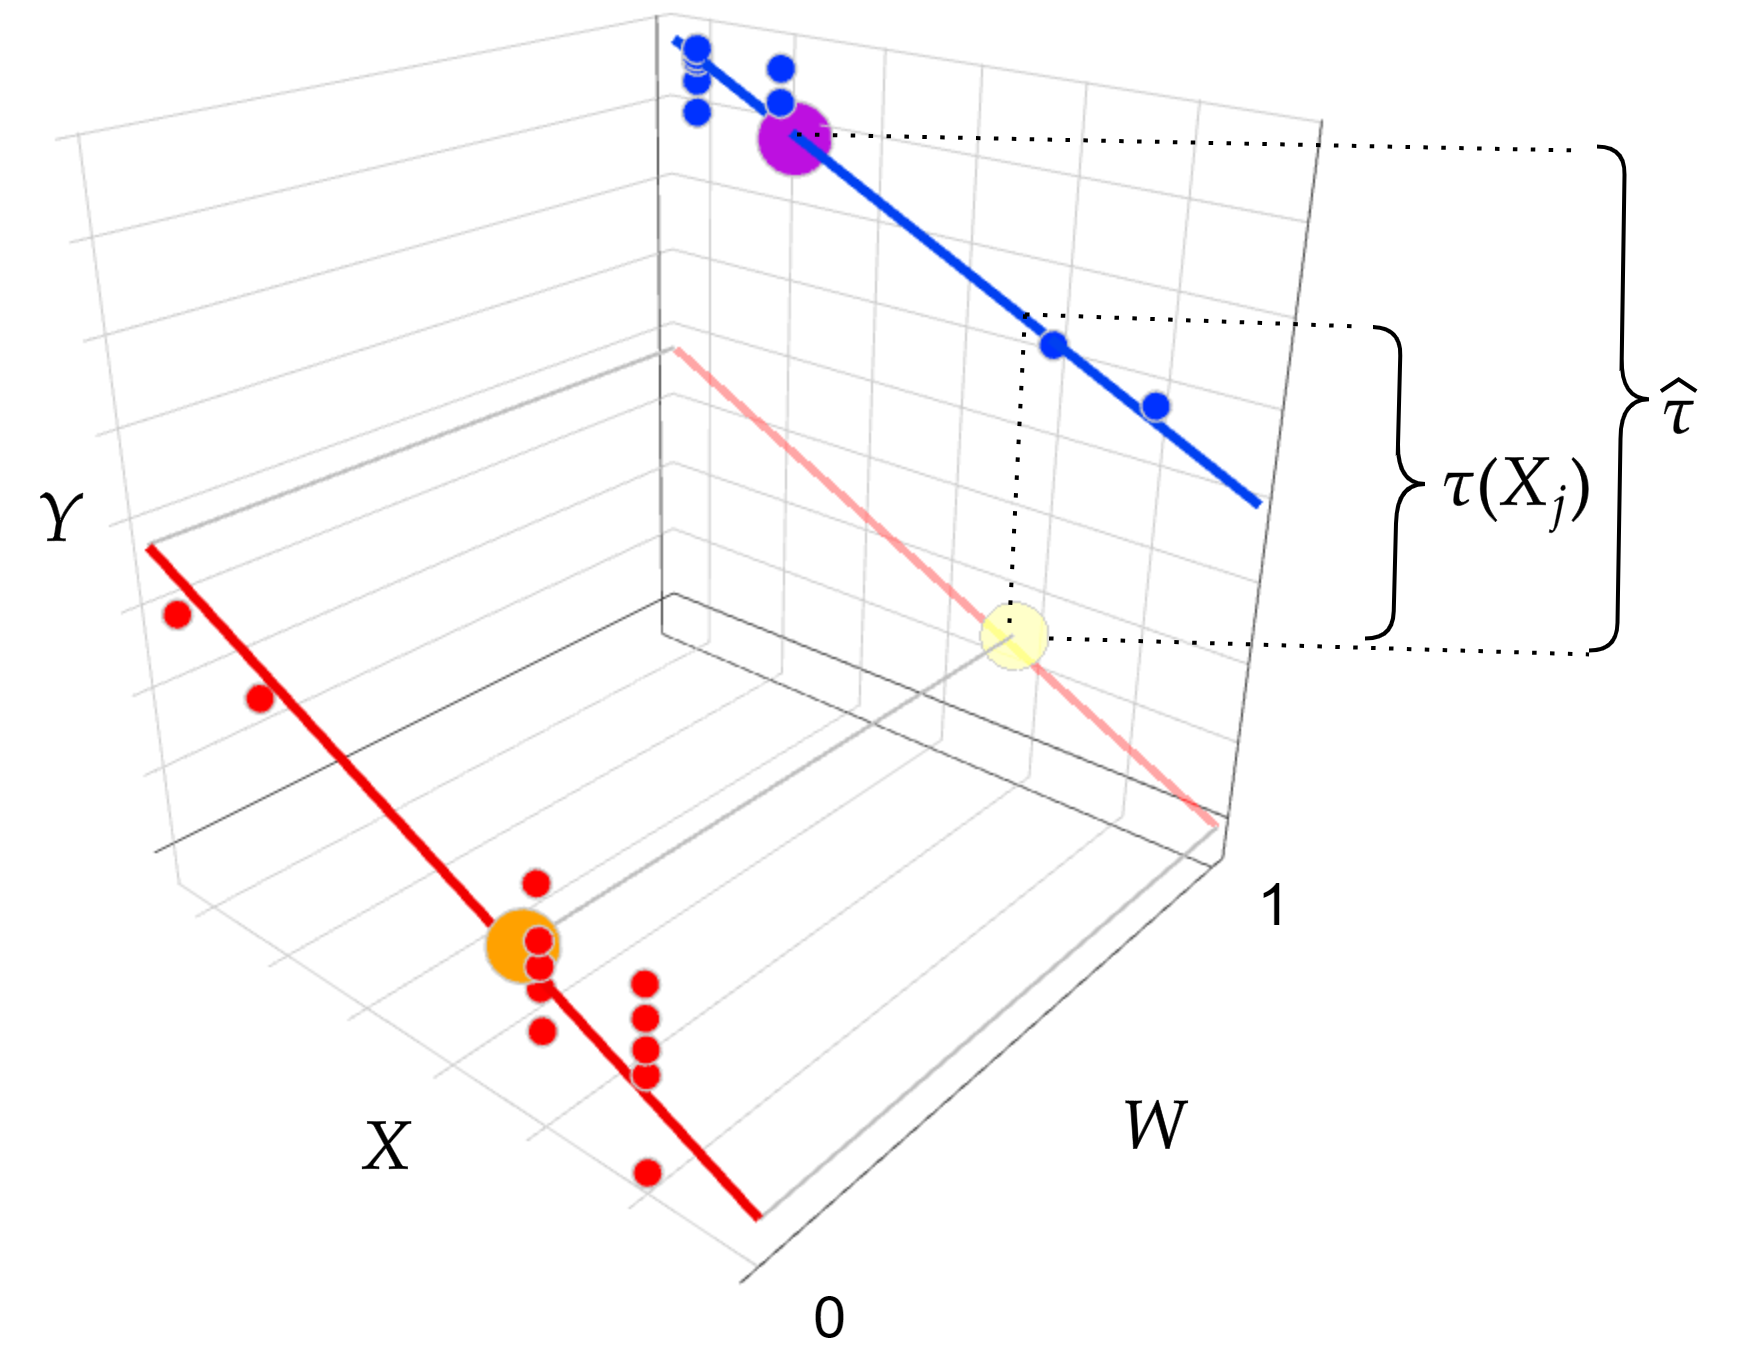
\includegraphics[width=0.55\linewidth]{sections/images/propensity.png}
    \caption{Illustration of covariate balance of propensity score (An example with linear dependence)}
\end{figure}

\begin{point}
    Statistical Inference to Propensity Score
\end{point}

Property of propensity score:
\begin{align*}
    \Delta _\mathrm{tc}:= \mathbb{E}\left[ e(X)|W=1 \right] - \mathbb{E}\left[ e(X) |W=0\right]=\dfrac{var(e(X))}{p(1-p)}\\
    var(e(X))=\mathbb{E}\left[ \left(\dfrac{f_\mathrm{t}(X)-f_\mathrm{c}(X)  }{pf_\mathrm{t}(X)+(1-p)f_\mathrm{c}(X)}\right)^2 \right]\cdot p^2(1-p)^2   
\end{align*}
\begin{itemize}[topsep=2pt,itemsep=0pt]
    \item Propensity Score test can be accessed by
\begin{align*}
    &\hat{\Delta }_\mathrm{tc}^\ell = \dfrac{\bar{\ell}_\mathrm{t}-\bar{\ell}_\mathrm{c}  }{\sqrt{(s^2_{\ell,\mathrm{t} }+s^2_{\ell,\mathrm{c} } )/2}}\sim t_{N-2},\quad \ell(x)=\ln\left(\dfrac{e(x)}{1-e(x)}\right)=\mathrm{logistic}(x) \\
    &\hat{\Delta }_\mathrm{tc}^\ell =0\leftrightsquigarrow \Delta _\mathrm{tc}=0\leftrightsquigarrow var(e(X))=0\leftrightsquigarrow f_\mathrm{t}(x)=f_\mathrm{c}(x)  
\end{align*}
    \item Estimate $ \hat{e}(X_i) $
    \begin{itemize}[topsep=2pt,itemsep=0pt]
        \item For categorical $ X $ with small $ |\mathcal{X}| $, estimation
        \begin{align*}
            \hat{e}(x)=\dfrac{N(X_j)}{N} 
        \end{align*}
        \item (Kernel) logistic regression is sometimes useful\footnote{Instruction of Kernel logistic regression see \autoref{SubSubSectionKernelRegression}.}
        \begin{align*}
             \hat{e}(x)=\hat{\mathbb{P}}\left( W_i=1|X_i=x;\beta  \right)=\dfrac{e^{x'\beta }}{1+e^{x'\beta }} 
        \end{align*}
    \end{itemize}
    
\end{itemize}

    







\begin{point}
    Useful Methods to Induce Propensity Score in Estimation
\end{point}
\begin{itemize}[topsep=2pt,itemsep=0pt]
    \item Weighting: using the modulation of $ e(x) $ on $ \mathbb{P}\left( W|X \right)  $
    \begin{align*}
        \begin{cases}
            \mathbb{E}\left[ \dfrac{Y_i^\mathrm{obs}\cdot W_i }{e(X_i)} \right]=\mathbb{E}\left[ \dfrac{\mathbb{E}\left[ Y_i(1)|X_i \right]\mathbb{E}\left[ W_i|X_i \right]  }{e(X_i)} \right]=\mathbb{E}\left[ Y_i(1) \right]\\
            \mathbb{E}\left[ \dfrac{Y_i^\mathrm{obs}\cdot (1-W_i) }{1-e(X_i)} \right]=\mathbb{E}\left[ \dfrac{\mathbb{E}\left[ Y_i(0)|X_i \right]\mathbb{E}\left[ 1-W_i|X_i \right]  }{1-e(X_i)} \right]=\mathbb{E}\left[ Y_i(0) \right]
        \end{cases} 
    \end{align*}
    to \textit{weight} estimators through $ X $: Horvitz-Thompson Estimator \index{Horvitz-Thompson Estimator}
    \begin{align*}
        \hat{\tau}^\mathrm{HT} = & \dfrac{1}{N}\sum_{i=1}^N\dfrac{W_iY^\mathrm{obs}_i }{\hat{e}(X_i)}-\dfrac{1}{N}\sum_{i=1}^N\dfrac{(1-W_i)Y^\mathrm{obs}_i }{1-\hat{e}(X_i)}=\dfrac{1}{N}\sum_{i=1}^N\dfrac{(W_i-e(X_i))\cdot Y^\mathrm{obs}_i }{e(X_i)\cdot (1-e(X_i))} \\
        \hat{\tau}^\mathrm{HT,mod} = & \sum_{i=1}^N \lambda _iW_iY^\mathrm{obs}_i-\sum_{i=1}^N\lambda _i(1-W_i)Y^\mathrm{obs}_i ,\quad \lambda _i=\begin{cases}
            \dfrac{1/\hat{e}(X_i)}{\sum_{k=1}^NW_i /\hat{e}(X_j)},&W_i=1\\
            \dfrac{1/(1-\hat{e}(X_i))}{\sum_{k=1}^N  (1-W_i)/(1-\hat{e}(X_k))},&W_i=0
        \end{cases}  
    \end{align*}
    where the modification version is used to avoid extreme $ \hat{e} $ value.

    The Horvitz-Thompson estimator is linked to stratified Neyman estimator \autoref{EqaNeymanEstimatorStratified} as
    \begin{align*}
         \hat{\tau}^\mathrm{strata}=\sum_{j=1}^Jq(j)\hat{\tau}(j)= \dfrac{1}{N} \sum_{i=1}^N \tilde{e} _iW_iY^\mathrm{obs}_i-\sum_{i=1}^N\tilde{e} _i(1-W_i)Y^\mathrm{obs}_i ,\quad \tilde{e} _i=\begin{cases}
            \mathbb{I}_{S_i=j}\dfrac{1}{N_\mathrm{t}(j)/N(j) },&W_i=1\\
            \mathbb{I}_{S_i=j}\dfrac{1}{N_\mathrm{c}(j/N(j)) },&W_i=0
         \end{cases}
    \end{align*}
    where $ \tilde{e }_i $ is the propensity score for each strata.
    \item Blocking / Stratifying according to $ X $, and then follows similar idea as SRE. (Because $ S(X_i) $ is still a covariate.)
    \item Matching `similar' data points. e.g. for each data point $ (W_i=1,Y_i,X_i) $, select in $ \mathcal{D}_{W=1-W_i=0} $ for units with small distance $ d(X_i,X) $ as $ \mathcal{M}_i $, and have a matching data
    \begin{align*}
        \{(W_i=1,Y_i^\mathrm{obs} ,X_i,\mathcal{M}_i)\},\quad \mathcal{M}_i=\{(W_j=0,Y_j,X_j)\}_{d(X_i,X_j)\text{ small}} 
    \end{align*}
    and then
    \begin{align*}
        \hat{\tau} =\dfrac{1}{N_\mathrm{t} }\sum_{i:W_i=1}\left(Y_i^\mathrm{obs}-\bar{Y}_{\mathcal{M}_i} \right)
    \end{align*}
\end{itemize}


\subsection{Pearl Bayesian Framework}
\index{Pearl Bayesian Framework}\index{Bayesian Network}\index{Belief Network}\index{DAG Model (Directed Acyclic Graphical Model)}
    Pearl Bayesian Framework\footnote{Also called Bayesian Network / Belief Network / Directed Acyclic Graphical (DAG) Model.} (Judea Pearl, 1995) uses causal information on a graph to construct inference. 













 \begin{center}
    \begin{minipage}{0.7\linewidth}
        \begin{align*}
            \mathbb{P}\left( X_1,X_2,X_3,X_4,X_5 \right) = & \mathbb{P}\left( X_5|X_4 \right) \mathbb{P}\left( X_1,X_2,X_3,X_4 \right) \\
            =&\mathbb{P}\left( X_5|X_4 \right) \mathbb{P}\left( X_4|X_2,X_3 \right) \mathbb{P}\left( X_1,X_2,X_3 \right) \\
            =&\mathbb{P}\left( X_5|X_4 \right) \mathbb{P}\left( X_4|X_2,X_3 \right) \mathbb{P}\left( X_3|X_1 \right) \mathbb{P}\left( X_2|X_1 \right) \mathbb{P}\left( X_1 \right)  \quad\,       
        \end{align*}
    \end{minipage}
    \begin{tikzpicture}[baseline={([yshift = 0ex]current bounding box.center)}]
        \GraphInit[vstyle=Dijkstra]
        \SetGraphUnit{1.2}
        
        \Vertices[Lpos=-45]{circle}{3,1,2,4}
        \SO[unit = 1.4](4){5}

        \tikzset{LabelStyle/.style={fill = white},
        EdgeStyle/.style={-stealth}}

        \Edge(1)(2)
        \Edge(1)(3)
        \Edge(3)(4)
        \Edge(2)(4)
        \Edge(4)(5)
      \end{tikzpicture}
    \end{center}




    
    \begin{center}
        \begin{minipage}{0.3\linewidth}
            \begin{figure}[H]
            \centering            
                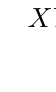
\begin{tikzpicture}[baseline={([yshift = -3ex]current bounding box.center)}]
                \GraphInit[vstyle=Dijkstra]
                \SetGraphUnit{0.8}
                \Vertex[x=0, y=0, L=$ X $]{1}
                \Vertex[x=1.5, y=0, L=$ Y $]{2}
                \Vertex[x=3, y=0, L=$ Z $]{3}

                \tikzset{LabelStyle/.style={fill = white},
                EdgeStyle/.style={-stealth}}
        
                \Edge(1)(2)
                \Edge(2)(3)
            \end{tikzpicture}            
            \caption{aa}
            \end{figure}
        \end{minipage}\quad\begin{minipage}{0.3\linewidth}
            \begin{figure}[H]
            \centering            
            \begin{tikzpicture}
                \GraphInit[vstyle=Dijkstra]
                \SetGraphUnit{0.8}
                \Vertex[x=0, y=0, L=$ X $]{1}
                \Vertex[x=1, y=1.73, L=$ Y $]{2}
                \Vertex[x=2, y=0, L=$ Z $]{3}

        
                \tikzset{LabelStyle/.style={fill = white},
                EdgeStyle/.style={-stealth}}
        
                \Edge(2)(1)
                \Edge(2)(3)
            \end{tikzpicture}        
            \caption{aa}
            \end{figure}
        \end{minipage}\quad\begin{minipage}{0.3\linewidth}
            \begin{figure}[H]
            \centering          
            \begin{tikzpicture}
                \GraphInit[vstyle=Dijkstra]
                \SetGraphUnit{0.8}
                \Vertex[x=0, y=0, L=$ X $]{1}
                \Vertex[x=1, y=-1.73, L=$ Y $]{2}
                \Vertex[x=2, y=0, L=$ Z $]{3}

        
                \tikzset{LabelStyle/.style={fill = white},
                EdgeStyle/.style={-stealth}}
        
                \Edge(1)(2)
                \Edge(3)(2)
            \end{tikzpicture}
            \caption{aa}
            \end{figure}
        \end{minipage}
    \end{center}

    \begin{center}
        \begin{minipage}{0.23\linewidth}
            \begin{figure}[H]
            \centering            
                \begin{tikzpicture}[baseline={([yshift = -3ex]current bounding box.center)}]
                    \GraphInit[vstyle=Dijkstra]
                    \SetGraphUnit{1.2}
                    
                    \Vertices[Lpos=-45]{circle}{3,1,2,4}
                    \SO[unit = 1.4](4){5}

                    \tikzset{LabelStyle/.style={fill = white},
                    EdgeStyle/.style={thick}}
            
                    \Edge(1)(2)
                    \Edge(1)(3)
            
                    \tikzset{LabelStyle/.style={fill = white},
                    EdgeStyle/.style={-stealth}}
            
                    \Edge(3)(4)
                    \Edge(2)(4)
                    \Edge(4)(5)
            \end{tikzpicture}     
            $$ \text{(part of) Skeleton} $$       
            % \caption{aa}
            \end{figure}
        \end{minipage}\quad
        \begin{minipage}{0.23\linewidth}
            \begin{figure}[H]
            \centering            
                \begin{tikzpicture}[baseline={([yshift = -3ex]current bounding box.center)}]
                    \GraphInit[vstyle=Dijkstra]
                    \SetGraphUnit{1.2}
                    
                    \Vertices[Lpos=-45]{circle}{3,1,2,4}
                    \SO[unit = 1.4](4){5}
            
                    \tikzset{LabelStyle/.style={fill = white},
                    EdgeStyle/.style={-stealth}}
            
                    \Edge(1)(2)
                    \Edge(1)(3)
                    \Edge(3)(4)
                    \Edge(2)(4)
                    \Edge(4)(5)
            \end{tikzpicture}     
            $$ G_1 $$       
            % \caption{aa}
            \end{figure}
        \end{minipage}\quad        \begin{minipage}{0.23\linewidth}
            \begin{figure}[H]
            \centering            
                \begin{tikzpicture}[baseline={([yshift = -3ex]current bounding box.center)}]
                    \GraphInit[vstyle=Dijkstra]
                    \SetGraphUnit{1.2}
                    
                    \Vertices[Lpos=-45]{circle}{3,1,2,4}
                    \SO[unit = 1.4](4){5}
            
                    \tikzset{LabelStyle/.style={fill = white},
                    EdgeStyle/.style={-stealth}}
            
                    \Edge(1)(2)
                    \Edge(3)(1)
                    \Edge(3)(4)
                    \Edge(2)(4)
                    \Edge(4)(5)
            \end{tikzpicture}  
            $$  G_2 $$        
            % \caption{aa}
            \end{figure}
        \end{minipage}\quad        \begin{minipage}{0.23\linewidth}
            \begin{figure}[H]
            \centering            
                \begin{tikzpicture}[baseline={([yshift = -3ex]current bounding box.center)}]
                    \GraphInit[vstyle=Dijkstra]
                    \SetGraphUnit{1.2}
                    
                    \Vertices[Lpos=-45]{circle}{3,1,2,4}
                    \SO[unit = 1.4](4){5}
            
                    \tikzset{LabelStyle/.style={fill = white},
                    EdgeStyle/.style={-stealth}}
            
                    \Edge(2)(1)
                    \Edge(1)(3)
                    \Edge(3)(4)
                    \Edge(2)(4)
                    \Edge(4)(5)
            \end{tikzpicture} 
            $$  G_3  $$
            % \caption{aa}
            \end{figure}
        \end{minipage}
    \end{center}



    \begin{center}
        \begin{tikzpicture}
            \GraphInit[vstyle=Dijkstra]
            \SetGraphUnit{0.8}
            
            \Vertex[x=4.5, y=2, L= $ X_1 $]{1}
            \Vertex[x=0, y=0, L=$ X_2 $]{2}
            \Vertex[x=3, y=-2, L=$ X_3 $]{3}
            \Vertex[x=6, y=0, L=$ X_4 $]{4}
            \Vertex[x=9, y=0, L=$ X_5 $]{5}
            \Vertex[x=3, y=-4, L=$ X_6 $]{6}
    
            \tikzset{LabelStyle/.style={fill = white},
            EdgeStyle/.style={-stealth}}
    
            \Edge(1)(2)
            \Edge(1)(5)
            \Edge(2)(3)
            \Edge(4)(3)
            \Edge(4)(5)
            \Edge(3)(6)
          \end{tikzpicture}
    \end{center}